\begin{frame}
  \frametitle{Binary relations are everywhere}
\vfill
  \begin{tabular}{M{5cm}M{5cm}}
    List of instructions:
    &
    \invisible<1>{Relation between memory states:\\}

    \begin{tabular}[t]{l}
    \texttt{\color{blue}cmd1;}\onslide<2>{$\color{red}\leftarrow$}\\

    \texttt{\color{darkgreen}cmd2;}\onslide<3>{$\color{red}\leftarrow$}\\

    \texttt{\color{orange}cmd3;}\onslide<4>{$\color{red}\leftarrow$}
    \end{tabular}

    &
\invisible<1>{
    \begin{tikzpicture}
    \coordinate (t) at (0,0);
    \onslide<1->{
      \node (t1) at (t) 
      {
\includegraphics[width=1.2cm]{db.png}};
      \node () at (t1) {1};
    }
    \onslide<3->{
      \node (t2) at ($(t1)-(0,2)$) 
      {
\includegraphics[width=1.2cm]{db.png}};
      \node () at (t2) {2};
    }
    \onslide<4->{
      \node (t3) at ($(t2)-(0,2)$) 
      {
\includegraphics[width=1.2cm]{db.png}};
      \node () at (t3) {3};
    }
    \onslide<5->{
      \node (t4) at ($(t3)-(0,2)$) 
      {
\includegraphics[width=1.2cm]{db.png}};
      \node () at (t4) {4};
    }
    \onslide<3->{\draw[blue,arc] (t1) to (t2);}
    \onslide<4->{\draw[darkgreen,arc] (t2) to (t3);}
    \onslide<5->{\draw[orange,arc] (t3) -- (t4);}
    \onslide<6>{\cedge[red][bend left] (t1)(t4);}
    \end{tikzpicture}}
  \end{tabular}
  \note{Our motivtion for this work comes from the task of verification of imperative programs. These programs are lists of instructions. A pleasant way to think about these prime instructions is a relations which transforms the memry states. For insatnce the blue operation can be seen as this blue relation etc. And the whole program can be seen as the composition of these relations. }
\end{frame}

\begin{frame}
\frametitle{Motivation: Verification of imperative programs}
\framesubtitle{Relational program semantics}
  \vfill
  \begin{tikzpicture}[xscale=3]
    \node (P) at (0,4) {${\color{red}x\leftarrow 1};\paren{\paren{{\color{darkgreen}y\leftarrow x}}\oplus\paren{{\color{blue}y\leftarrow 0}}}$};
    \node (P') at (2,4) {$\paren{{\color{red}x\leftarrow 1};{\color{darkgreen}y\leftarrow x}}\oplus 
      \paren{{\color{red}x\leftarrow 1};{\color{blue}y\leftarrow 0}}$};
    
    \onslide<2->{
      \node (e) at (0,3) {${\color{red}a}\cdot({\color{darkgreen}b}\cup {\color{blue}c})$};
      \node (e') at (2,3) {$({\color{red}a}\cdot {\color{darkgreen}b})\cup({\color{red}a}\cdot {\color{blue}c})$};}
    \onslide<2>{
      \draw[|->,thick] (P) -- (e);
      \draw[|->,thick] (P') -- (e');
    }
    
    \onslide<3->{
      \node (eqe) at ($(e.east)!.5!(e'.west)$) {$=$};
      \node (ka) at ($(e)-(1,0)$) {$\Rel$};
      \node (vd) at ($(ka.east)!.5!(e.west)$) {$\models$};
    }
    
    \onslide<4->{
      \node (eqP) at ($(P.east)!.5!(P'.west)$) {$\equiv$};
    }
    
  %  \onslide<5->{
  %    \node (eqe) at ($(e.east)!.5!(e'.west)$) {$\subseteq$};
  %    \node (ka) at ($(e)-(1,0)$) {$\Rel$};
  %    \node (vd) at ($(ka.east)!.5!(e.west)$) {$\models$};
  %  }
    
  %  \onslide<6->{
  %    \node (eqP) at ($(P.east)!.5!(P'.west)$) {$\preceq$};
  %  }
  \end{tikzpicture}
\vfill
\onslide<5->{
\begin{minipage}{.35\linewidth}

    \begin{block}{Relational Operators} 
      \onslide<+->{}
      \begin{tabular}        {>{\color{basecolor!80!black}}l@{~~}>{\centering\arraybackslash\textcolor{black}}c@{$~$}l}
        Identity relation
        & $\Un$\\
        Empty relation
        & $\Zero$
        \\
        Composition 
        & $R\cdot S$\\
        Union 
        & $R\cup S$\\
        Iteration & $R^+$\\
        Intersection 
        & $R\cap S$\\
        Converse & $\conv{R}$\\
        Compement & $R^c$\\
        $\vdots$ &\\
      \end{tabular}%
    \end{block}
\end{minipage}}
\onslide<6->{
\begin{minipage}{.5\linewidth}
\begin{itemize}
\item \textbf{\KA$\ $  operators:} $$\Un\ \mid\ \Zero\ \mid\ R\cdot S\ \mid\  R\cup S\ \mid\ R^+$$
\item \textbf{\KLm$\ $ operators:} $$\Zero\ \mid\ R\cdot S\ \mid\  R\cup S\ \mid\ R^+\ \mid \ R\cap S$$
\onslide<7>{\item \textbf{Example of a universal law:} 
$$\Rel\models (R \cap S)\cdot T \subseteq (R \cdot T) \cap (S \cdot T)$$
\end{itemize}}
\end{minipage}
}
\note{\only<1-6>{Now if our problem is to check that two imperative programs have the same behaviour, one possible way to proceed is to abstract these instructions into relations (here a, b and c) and check that the obtained expressions are equal in the relational model. This means that no matter how we chose to interpret a, b, c as relations, the equation still hold. If this is the case, we can be sure that the two programs have the same behaviour.  } \only<7->{In this example, we used relations composion and union to simulate programs composition and non-deterministic choice. But depending on the class of programs under consideration, we may need other operators, for instance transitive closure to simulate while loop, (et les autres? ) In this presentation I will focus on two classes of operators: the first one is the set of KA operators. If we look at the expressions generated by these operations we get regular expressions. This class of operators is very standard, and will serve as a reference point.
The second class of operators are the KLm operators. It contains the operators of KA except the identity(1) together with the intersection operator. And I introduce it because my completness result will be about this fragment.  
Here is an example of a valid law in KLm. Note that in the first law I considered the equality relation, while I considered inclusion in the second one. Both are interesting. 

 }

}
\end{frame}

\begin{frame}
  \frametitle{Two important properties  about $ \Rel \models e \subseteq f$ }
\vspace{.7cm}
    \begin{minipage}{.4\linewidth}
\begin{center}    
    \textbf{Decidability} \\
      \vspace{.7cm}
      \begin{tikzpicture}[->,>=stealth',shorten >=1pt,auto,
                    thick]
        \tikzstyle{state}=[draw]
        
  \node[draw=none](A) at (1.5,-2.5) {
    {\color{red}$\overset{?}{\Rel\models e \subseteq f }$}};  
  \node[state, rounded corners=5, fill=yellow!10] (TS) at (0,-2)  {\scriptsize Expression $e$};
  \node[state, rounded corners=5, fill=yellow!10] (MCF) at (3,-2)  {\scriptsize Expression $f$};  
  \node[state, rounded corners=5, fill=blue!10](MC) at (1.5,-4) {\scriptsize Algorithm};
  \node[draw=none](A) at (1.5,-5) {\scriptsize \textbf{YES/NO}};
\node[draw=none](Aa) at (1.5,-5.5) {\scriptsize \textbf{(Boolean answer)}};

  \path 
        (TS) edge     node{} (MC)
        (MCF) edge      node{} (MC)
        (MC) edge      node{} (A);  
\end{tikzpicture}
        \end{center}
    \end{minipage}
$\qquad$
    \begin{minipage}{.4\linewidth}
\begin{center}    
    \textbf{Axiomatizability}\\ 
 \vspace{.7cm}
      \begin{tikzpicture}[->,>=stealth',shorten >=1pt,auto,
                    thick]
        \tikzstyle{state}=[draw]
        
  \node[draw=none](A) at (1.5,-2.5) {
    {\color{red}$\overset{?}{\Rel\models e \subseteq f }$}};  
  \node[state, rounded corners=5, fill=yellow!10] (TS) at (0,-2)  {\scriptsize Expression $e$};
  \node[state, rounded corners=5, fill=yellow!10] (MCF) at (3,-2)  {\scriptsize Expression $f$};  
  \node[state, rounded corners=5, fill=blue!10](MC) at (1.5,-4) {\scriptsize Axioms};
  \node[draw=none](A) at (1.5,-5) {\scriptsize \textbf{Proof/counter-example}};
\node[draw=none](Aa) at (1.5,-5.5) {\scriptsize \textbf{(Certificate)}};

  \path 
        (TS) edge     node{} (MC)
        (MCF) edge      node{} (MC)
        (MC) edge      node{} (A);  
\end{tikzpicture}
        \end{center}    
    \end{minipage}
    \vfill\onslide<2->{
    \begin{block}{$\qquad\qquad\qquad\quad$ Decidability $\qquad\qquad$ Axiomatizability  }
\begin{center}    
    \begin{tabular}{c|c|c}
    KA $\quad$ & PSPACE-complete  & Kleene Algebra  \\[10pt] 
    \KLm $\quad$ & EXPSPACE-complete  & \only<1,2>{$\qquad\qquad\qquad$\textbf{?}$\qquad\qquad\qquad$} \only<3>{\textbf{Identity free Kleene Lattices}}\\ 
    \end{tabular}
    \end{center}
    \end{block}}%\vfill
%    \begin{enumerate}
 %   \item[(1)]   \simplecite{Pratt}{Dynamic algebras and the nature of induction}{1980}
 %   \item[(2)]   \simplecite{ Kozen}{A completeness theorem for Kleene algebras}{1994}
  %  \item[(3)]   \simplecite{ Brunet \& Pous}{Petri automata for Kleene Allegories}{LICS'15}
    
   % \end{enumerate
    \note{To use this relational semantics in verification, one should obtain two propetries. The first is decidability of the relational equivalence of two expressions e and f, and the second is its axiomatisatbility. Decidability makes it possible to automate the verification process, while axiomatizability provides a certificate for programs
verification. Indeed, an axiomatic proof of e = f can be seen as a certificate, which can
be exchanged, proofread, and combined in a modular way. 

Here is a summary of the situation of the KA and KL fragments. We know that the equational theory of KA is decidable, it is even PSPACE-complete,  it admits a finite axiomatisation which is just the axioms of Kleene Algebra.
We know also that KL is EXPSPACE complete.  
What is missing to this picture is an axiomatisation of KL. 


A garder en tete:
la reference a Pratt est ok, mais il faut bien avoir conscience
que Pratt prouve Rel|=e=f <-> [e]=[f], pas le resultat de complexite
(qui est du à Kleene puis Meyer et Stockmeyer) la ref a Kozen est ok, mais a nouveau il ne faut pas que tu
oublies Boffa et Krob si on te pose une question
}\end{frame}















\section{Overview on \KA}
%\subsection{Regular expressions}
%\subsection{Axiomatization}

%\frame{\frametitle{Outline}\tableofcontents}
%\frame{\frametitle{Outline}\tableofcontents[currentsection]}
\begin{frame}
  \frametitle{Regular expressions \& languages}
  
  Let $\Sigma=\set{a,b,\dots}$ be a finite alphabet.

  \begin{block}{Regular expressions}
    \[e,f\in\reg\Coloneqq \Zero\Mid\Un\Mid a\Mid e\cdot f\Mid
      e\cup f\Mid e^+\]
  \end{block}
  \vfill\pause
  \begin{exampleblock}{Examples}\vspace{-0.5cm}
    \begin{align*}
      &\lang{a\cdot(b\cup c)}=\set{ab,ac}&&\lang{a\cdot\Zero}=\emptyset\\
      &\lang{a^+}=\set{a,aa,\dots}=\setcompr{a^n}{n\in\Nat}
    \end{align*}
  \end{exampleblock}
  \pause 
  \vfill
  \begin{theorem}[Pratt 1980]
  $$\Rel \models e\subseteq f\  \Leftrightarrow\ \lang{e}\subseteq \lang{f}$$
  Where $\lang{e}$ is the rational language of the expression $e$.
  \end{theorem}
\note{Before showing this axiomatization, let us have a quick look at the KA fragment.
The KA expressions are what we usually call regular expressions. To each regular expression we can associate a language of words that we denote by L(e), which charachetrizes the relational equivalence between two expressions. This charachterization theorem can be used to establish the decidability of the theory, if we use the kleene theorem. This theorem says that every expression is equivalent to an NFA, thus checking e<f in rel amounts to check language inclusion of two NFA, which is decidable.}

\end{frame}

\newsavebox{\bototomates}\sbox{\bototomates}{%
  \begin{minipage}{.35\linewidth} \centering 
    \begin{tikzpicture}
      \node[state,initial,accepting below,minimum height=3ex] (0) {};
      \node[state,accepting below,minimum height=3ex] (1) [right of=0] {};
      \path[->] (0) edge node [above] {$a$} (1)
      edge [uploop] node [above] {$b$} ()
      (1) edge [uploop] node [above] {$b$} ();
    \end{tikzpicture}
%
 %   \vspace{1cm}

  %  \begin{tikzpicture}
   %   \node[state,initial,minimum height=3ex] (0) at (0,0) {};
    %  \node[state,minimum height=3ex] (1) at (1,1) {};
     % \node[state,minimum height=3ex] (2) at (1,-1) {};
      %\node[state,accepting right,minimum height=3ex] (3) at (2,0) {};
      %\path[->] 
      %(0) edge[out=60,in=-150] node [lbl] {$a$} (1)
      %edge [out=-60,in=150] node [lbl] {$b$} (2)
%      (1) edge [out=-30,in=120] node [lbl] {$b$} (3)
 %     edge [out=-120,in=30] node [lbl] {$a$} (0)
  %    (2) edge [out=30,in=-120] node [lbl] {$a$} (3)
   %   edge [out=120,in=-30] node [lbl] {$b$} (0)
    %  (3) edge [out=-150,in=60] node [lbl] {$a$} (2)
     % edge [out=150,in=-60] node [lbl] {$b$} (1);
    %\end{tikzpicture}
     \hfill
    \begin{minipage}{.8\linewidth}\centering
      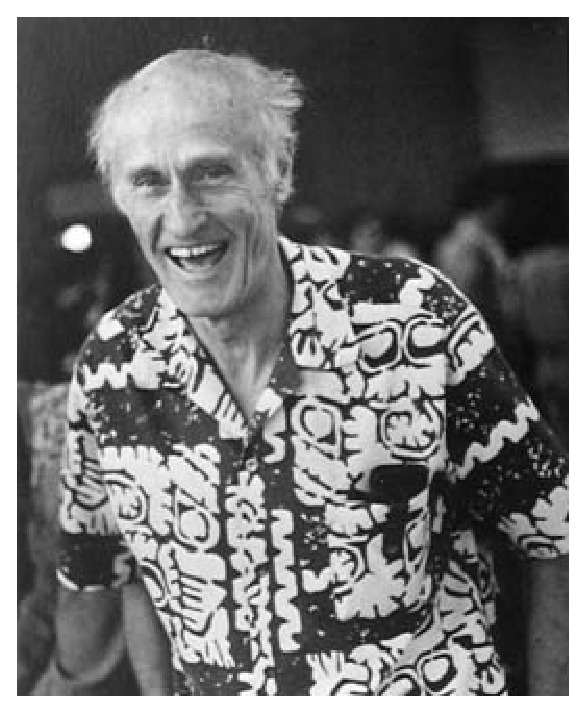
\includegraphics[width=1.0\linewidth]{kleene.eps}

      Stephen Cole Kleene
    \end{minipage}
  \end{minipage}
}
\newsavebox{\sck}\sbox{\sck}{%
  \begin{minipage}{.35\linewidth}
    \hfill
    \begin{minipage}{.8\linewidth}\centering
      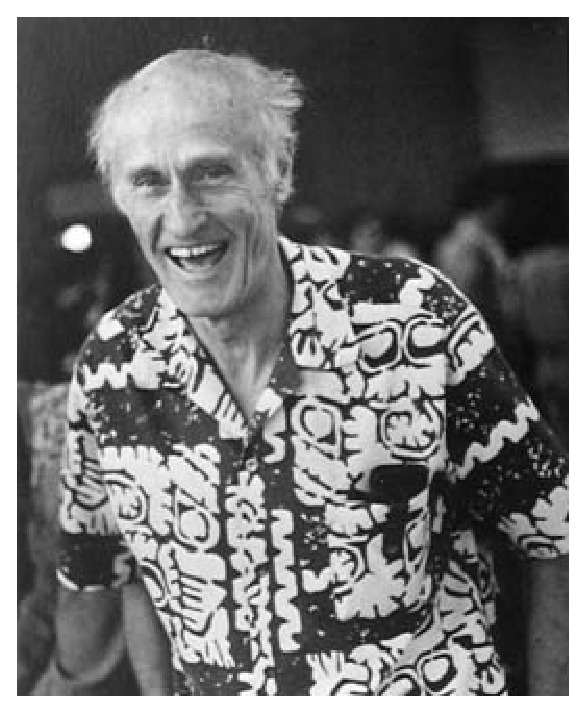
\includegraphics[width=1.0\linewidth]{kleene.eps}

      Stephen Cole Kleene
    \end{minipage}
  \end{minipage}
}

\begin{frame}
  \frametitle{Non-deterministic Finite Automata (NFA)}
  \begin{minipage}{.6\linewidth}
    \onslide<2->{
      \begin{block}{Kleene Theorem}
         A language is regular if and only if it is recognised by a NFA.
      \end{block}} 
    \vspace{.5cm}
 \onslide<3->{
      \begin{block}{Theorem}
        Automata equivalence is decidable.
      \end{block}} 
    \vspace{.5cm}
    \onslide<4->{
\begin{block}{Corollary}
Relational equivalence is decidable for regular expressions.
      \end{block}}
  \end{minipage}%
 %  {\usebox{\bototomates}}%<2->{\usebox{\sck}}
 \begin{minipage}{.35\linewidth} \centering 
    \begin{tikzpicture}
      \node[state,initial,accepting below,minimum height=3ex] (0) {};
      \node[state,accepting below,minimum height=3ex] (1) [right of=0] {};
      \path[->] (0) edge node [above] {$a$} (1)
      edge [uploop] node [above] {$b$} ()
      (1) edge [uploop] node [above] {$b$} ();
    \end{tikzpicture}

    \vspace{1cm}

    \begin{tikzpicture}
      \node[state,initial,minimum height=3ex] (0) at (0,0) {};
      \node[state,minimum height=3ex] (1) at (1,1) {};
      \node[state,minimum height=3ex] (2) at (1,-1) {};
      \node[state,accepting right,minimum height=3ex] (3) at (2,0) {};
      \path[->] 
      (0) edge[out=60,in=-150] node [lbl] {$a$} (1)
      edge [out=-60,in=150] node [lbl] {$b$} (2)
      (1) edge [out=-30,in=120] node [lbl] {$b$} (3)
   edge [out=-120,in=30] node [lbl] {$a$} (0)
    (2) edge [out=30,in=-120] node [lbl] {$a$} (3)
     edge [out=120,in=-30] node [lbl] {$b$} (0)
      (3) edge [out=-150,in=60] node [lbl] {$a$} (2)
      edge [out=150,in=-60] node [lbl] {$b$} (1);
    \end{tikzpicture}
\hfill
     
  \end{minipage}
  \note{Regular languages, which are the languages of regular expressions, can be charachterizd by means of machines, the well know NFA. 
  We have have this Kleene thm which says that a langage is regular iff it is recognized by an NFA.
  
  NFA have this pleasant property that  }
\end{frame}


\begin{frame}
  \frametitle{Axiomatization}
  \begin{block}{Axioms of Kleene Algebra}
%  A Kleene algebra is an algebraic structure
 % $\langle K,\cup,\cdot,^\star,\Zero,\Un\rangle$ such that $\langle K,\cup,\cdot,\Zero,\Un\rangle$ is
  \begin{itemize}
  \item  Axioms of an idempotent
    semiring decribing the behaviour of $\cup,\cdot,\Zero,\Un$.
  \item Two axioms describing the behaviour of $^+$: 
    $$\begin{array}{c}
    f\cdot e \cup f \leq f \quad\Rightarrow\quad f \cdot e^+ \cup f \leq f\\
    e\cup e\cdot e^+ \leq e^+ 
    \end{array}$$
  \end{itemize}
  \vfill
  \begin{center}
\textbf{We write $\text{\KA} \vdash e \leq f$ \\if $e\leq f$ follows from the axioms of Kleene Algebra.}
  \end{center}
  \end{block}
  \vfill
  \begin{theorem}[\only<2>{Soundness}\only<3,4>{Completeness}\only<1>{Kozen 1994}]
    $$\Rel \models e \subseteq f 
\only<1>{\quad \Leftrightarrow\quad}
\only<2>{\quad \Leftarrow\quad}  
\only<3>{\quad \Rightarrow\quad}
  \only<4>{\quad \Leftrightarrow\quad \lang{e}\subseteq\lang{f} \quad \Rightarrow\quad}
   \text{\KA} \vdash  e \leq f$$
  \end{theorem}

\vfill
\note{The relational equivalence (implication?) of two KA expressions can be axiomatized by the laws of Kleene algebra. 

These laws contain the laws of an ISR describing the behaviour of .. together with some laws for the star, reflecting the fact that it is a least fixed point. I am not going to give the details of this axiomatisation because they will not be important for us. We will just write KA proves e less than f if this inequality is provable from the axioms of Kleene algebra. 

Kozen showed that this axiomatization is sound and complete. Soundness which is the right to left implication is easy. The other implication is more complex, and here Kozen used again the charachterization of relational equivalence by language inclusions. To show that language inclusion implies provability, he used autoamta again, more precisely he reflected the language inclusion of the two automata correponding to e and f into KA. We will use similar ideas in our proof. }
\end{frame}

%\section{Overview on \KLm}
%\frame{\frametitle{Outline}\tableofcontents[currentsection]}

%\subsection{Expressions and graph languages}

\begin{frame}{\KLm$\ $ expressions and axiomatization}
  \[e,f\in\ireg\Coloneqq \Zero\Mid{\color{lightgray}\Un\Mid} a\Mid e\cdot f\Mid\bm{e\cap f}\Mid e\cup f\Mid e^+\]
  \vfill\onslide<2->{
\begin{block}{Axioms of identity-free Kleene lattices}
  \begin{itemize}
  \item Axioms of Kleene algebra.
  \item Axioms of a distributive lattice describing the behaviour of $\cup, \cap$.
  \end{itemize}
  \vfill
  \begin{center}
\textbf{We write $\text{\KLm} \vdash e \leq f$\\ if $e\leq f$ follows from the axioms of identity-free Kleene lattices.}
  \end{center}  \end{block}}
  \vfill
\onslide<3->{  \begin{theorem}
  $$\Rel \models e \subseteq f \quad \Leftrightarrow \quad \text{\KLm} \vdash  e \leq f$$
  \end{theorem}}
  \note{Let us go back to our axiomatization. As a reminder, here is the sytax ouf our KL expressions, we added intersection to the KA operators and removed one.
  The axioms we consider are those of Kleene algebra together with the axioms of a distributive lattice, describing how $\cup$ and $\cap$ behave. We write KL proves e less f 
  if this inequality follows from these axioms. 
  
  And we claim that these axiomatization is sound and complete.}
\end{frame}

\begin{frame}{Soundness and completeness}
\begin{theorem}[Soundness]
  $$\Rel \models e \subseteq f \quad \Leftarrow \quad \text{\KLm} \vdash  e \leq f$$
  \end{theorem}
\vfill
Check that every \KLm$\ $ axiom holds in $\Rel$.
\vfill
\onslide<2->{ \begin{theorem}[Completeness]
  $$\Rel \models e \subseteq f  
  \only<2>{\quad\Rightarrow\quad}
  \only<3>{\quad\Leftrightarrow\quad \lang{e}\subseteq \lang{f} \quad \Rightarrow\quad}\only<4,5,6>{\quad{\color{red}\nLeftarrow} \quad \lang{e}\subseteq \lang{f} \quad{\color{red}\nRightarrow}}\quad  \text{\KLm} \vdash  e \leq f$$
  \end{theorem}}
  \onslide<5,6>{$$\lang{a\cap b}\subseteq \lang{0}\qquad \text{ but }\qquad \Rel \nmodels a\cap b \leq 0\qquad\text{ and }\qquad \text{ \KLm }\nvdash a\cap b \leq 0$$}
\onslide<6>{
\begin{center}
\textbf{Another notion of language is needed!}
\end{center}}
\note{As before, soundness is not very difficult, it is enough to ckeck that every axiom holds in Rel.

Completeness is more difficult and the rest of the presentation will be dedicated to its proof. We are very tempted to do as Kozen did, and introduce language inclusion as intermediary step. The problem is that this characterization theorem, does not hold in presence of intersection. For instance, we have that, Lan(a inter b) = Lan (0) however, it is not true that Rel a inter b =0 nor KL a inter b =0. This means that this notion of language is not the right one in presence of intersection.  }
\end{frame}

\begin{frame}{Language of a KL expression}
\vfill 
  \centering
      \begin{tabular}{>{\hfill}m{3cm}@{:}>{\centering\arraybackslash}m{5cm}}
        $\G\paren{a\cdot b}$&
        \begin{tikzpicture}[baseline=(bl),scale=.6]
          \position(0)(0,0);
          \coordinate (bl) at ($(0)-(0,.3)$);
          \position(1)(1.5,0);
          \position(2)(3,0);
          \initst (0);
          \fnst (2);
          \edge[above] (0) (1)[a];
          \edge[above] (1) (2)[b];
        \end{tikzpicture}\\ \pause
        $\G\paren{a\cap b}$&   \begin{tikzpicture}[baseline=(bl), scale=.6]
          \position(a)(0,0); 
          \coordinate (bl) at ($(a)-(0,.3)$);
          \position(c)(1.5,0);
          \initst (a); \fnst (c); 
          \edge[above,out=35,in=145] (a) (c)[a]; 
          \edge[below,out=-35,in=-145] (a) (c)[b];
        \end{tikzpicture}\\ \pause 
        $\G\paren{\paren{a\cdot b}\cap\paren{c\cdot b}}$ &
        \begin{tikzpicture}[baseline=(bl), scale=.6]
          \position(a)(0,0); 
          \coordinate (bl) at ($(a)-(0,.3)$);
          \position(b1)(1.5,0.35); 
          \position(b2)(1.5,-0.35); 
          \position(c)(3,0);
          \initst (a); \fnst (c); 
          \edge[above,out=35,in=180] (a) (b1)[a]; 
          \edge[below,out=-35,in=180] (a) (b2)[c];  
          \edge[above,out=0,in=145] (b1) (c)[b];
          \edge[below,out=0,in=-145] (b2) (c)[b];
        \end{tikzpicture}\\
        \pause
        $\G\paren{\paren{a\cap b}^+}$ & $\set{ 
        \begin{tikzpicture}[baseline=(bl), scale=.6]
          \position(a)(0,0); 
          \coordinate (bl) at ($(a)-(0,.3)$);
          \position(c)(1.5,0);
          \initst (a); \fnst (c); 
          \edge[above,out=35,in=145] (a) (c)[a]; 
          \edge[below,out=-35,in=-145] (a) (c)[b];
        \end{tikzpicture}, 
        \begin{tikzpicture}[baseline=(bl), scale=.6]
          \position(a)(0,0); 
          \coordinate (bl) at ($(a)-(0,.3)$);
          \position(c)(1.5,0);
          \position(d)(3,0);
          \initst (a); \fnst (d); 
          \edge[above,out=35,in=145] (a) (c)[a]; 
          \edge[below,out=-35,in=-145] (a) (c)[b];
           \edge[above,out=35,in=145] (c) (d)[a]; 
          \edge[below,out=-35,in=-145] (c) (d)[b];
        \end{tikzpicture}, \dots}$
      \end{tabular}      
\vfill
\note{The language of an expression will be a set graphs instread of set of words. 
 Composition is interpeted as usual by a series composition, and intersection by a parallel composition as you can see in these two examples. Here is a more complex example: we did a series composition of a and b then a series composition of a and c, then we parral compose them to get this graph. When we have expressions with iteration, the interpretation will be a set of graphs instead of a single graph. For example, the interpretation of the iteration of a inter b, is the graph of a inter b, then the composition of the graph of a inter b twice etc. }
\end{frame}



\begin{frame}{Characterization theorem}\vspace{-10pt}
\only<1>{
    \begin{mathpar}
      \Rel\models e \subseteq f~\qmequiv~\G(e)\subseteq\G(f)
    \end{mathpar}}
    \only<2->{
    \begin{mathpar}
      \Rel\models e \subseteq f~\alert{\nRightarrow}~\G( e)\subseteq\G( f)
      \end{mathpar}}
      \vfill
\invisible<1,2>{
\textbf{Example:} $\qquad\quad\Rel \models  \paren{a\cap b}\cdot c \subseteq \paren{a\cdot c}\cap \paren{b\cdot c}$     
  \begin{center}
    \begin{tikzpicture}
%      \node (lblG) at (-3,0) {$G:$};
 %     \node (lblH) at (-3,2) {$H:$};
      \tikzstyle{arc}=[thick,->,>=latex]
      \tikzstyle{vert}=[thick,draw,circle,fill=gray!20]
      \position(0)(0,0); 
      \position(1)(1.5,0); 
      \position(2)(3,0);
      \initst (0); \fnst (2); 
      \edge[above,out=30,in=150] (0) (1)[a]; 
      \edge[below,out=-30,in=-150] (0) (1)[b]; 
  %    \edge[below,out=-40,in=-140] (0) (2)[d];
      \edge[above] (1) (2)[c]; 

      \position(x)(0,2);
      \position(y)(1.5,2.5); 
      \position(z)(1.5,1.5);
      \position(t)(3,2); 
      \initst (x); \fnst (t);
      \edge[above,out=50,in=180] (x) (y)[a]; 
      \edge[below,out=-50,in=180] (x) (z)[b];  
      \edge[above,out=0,in=130] (y) (t)[c];
      \edge[below,out=0,in=-130] (z) (t)[c];
\onslide<4->{
      \draw[arc,color=red,style=dotted] (x) to[bend right] (0);
      \draw[arc,color=red,style=dotted] (y) to[bend left] (1);
      \draw[arc,color=red,style=dotted] (z) to[bend right] (1);
      \draw[arc,color=red,style=dotted] (t) to[bend left] (2);
}
      \node (u) at (6,2) {$\paren{a\cdot c}\cap \paren{b\cdot c}$};
      % \node[rotate=-90] (trig) at (6,1) {$\lhd$};
      \node (v) at (6,0) {$\paren{a\cap b}\cdot c$};
    \end{tikzpicture}
  \end{center}}
  \onslide<4->{ 
      $G\lessgr H$ if there exists a graph homomorphism from $H$ to $G$.}
 \vfill
\onslide<5->{  \begin{block}{Theorem [Brunet \& Pous, LICS 2015]}
    %$e,f\in \areg,$
    $\clgr S$ is the downwards closure of $S$ with respect to $\lessgr$.
    \[\Rel\models e\subseteq f\Leftrightarrow \clgr{\G(e)}\subseteq
    \clgr{\G(f)}\]\vfill
  \end{block}
  \vfill}
\note{At this stage, we can ask whether we have our charachterization theorem. Well, this is still not the case. Take for instance this inequation which is valid in Rel. As you can see, the of graph of a inter b c is different from the graph of a b inter a c. Note however that there is graph homomorphism from the former to the later. A graph hohomorphism is a function that maps the nodes of a graph to the nodes of another such that if there is an edge between two nodes of the first graph labeled a, there is an edge labeled a between the images of these two nodes. (Comment dire ça de manière plus concise?)
  % 
  DAMIEN: je n'essaierai pas d'être plus concis, c'est bien de laisser le temps de digérer...
  suggestion ci-dessous:
  % 
  ... from the former to the later. That is, a function between the two sets of nodes that preserves edges and labels. For instance, the edges labelled with $c$ in the graph on the top are mapped to an edge with the same label in the graph below.
  % 
  % 
  Using this notion of homomorphism, we can have our characterization theorm: e  is less than f holds in the relational model iff the graph language of e is inclusded in the closure of the graph language of f by homomorphism. }
\end{frame}

%\subsection{Petri automata}
%\frame{\frametitle{Outline}\tableofcontents[currentsubsection]}

\begin{frame}{Completeness}
  \vfill
  \begin{theorem}[Completeness]
  $$\only<1>{\Rel \models e \subseteq f}\only<2->{\clgr{\G(e)}\subseteq\clgr{\G(f)}}\quad \Rightarrow \quad \text{\KLm} \vdash  e \leq f$$
  \end{theorem}
  \vfill
  \onslide<4>{\begin{center}
  \textbf{Need acceptors for these graph languages!}
  \end{center}}
\onslide<3->{  \begin{theorem}[Completeness for strict inclusions]
  $$\G(e) \subseteq \G(f) \quad \Rightarrow \quad \text{\KLm} \vdash  e \leq f$$
  \end{theorem}
  \begin{center}
 A strengthening of \KA$\ $ completeness with uninterpreted symbols.
  \end{center}
  }  
  \note{Now let us go back to our completeness result, whcih this time can be stated this way using the characterization theorem. 
  
  There is weak form of this theorem, which is easy to show and which will be useful later. It is completeness for strict language inclusions, whithout closure by graph homomorphism.  
  
But to show the general result, we will proceed as Kozen, and reflect some automata constructions by proofs. But for that we need a notion of automata for graph languages.   
  }
\end{frame}


\begin{frame}
  \frametitle{Petri automata}
\begin{itemize}
\item \textbf{Petri automaton:} 
\vspace{-.4cm}
  \begin{center}
  \scalebox{.6}{
  \begin{tikzpicture}
    \etat[i] (0) (0,0);\initst(0);
    \trans (t0) ($(0)+(2,0)$);
    \etat[1] (1) ($(t0)+(2,.5)$);
    \etat[2] (2) ($(t0)+(2,-.5)$);
    \trans (t1) ($(1)+(0,2)$);
    \transf(t4) ($(1|-2)!.5!(1)+(2,0)$);
    \edge(0)(t0);
    \edge[bend left,above](t0)(1)[a];
    \edge[bend right,below](t0)(2)[b];
    \edge[out=50,in=0](1)(t1);
    \edge[out=180,in=130,left](t1)(1)[c];
    \edge[out=0,in=130](1)(t4);
    \edge[out=0,in=-130](2)(t4);
      \end{tikzpicture}}
      \end{center}
\item \textbf{Graph language:} $\G(P)= \text{Graphs extracted from the runs of P}$
\pause
\item \textbf{Example:}
\begin{center}
  \scalebox{.8}{
  \begin{tikzpicture}
    \etat[i] (0) (0,0);\initst(0);
    \trans (t0) ($(0)+(1.5,0)$);
    \etat[1] (1) ($(t0)+(1.5,.5)$);
    \etat[2] (2) ($(t0)+(1.5,-.5)$);
    \transf(t4) ($(1|-2)!.5!(1)+(1.5,0)$);
    \edge(0)(t0);
    \edge[bend left,above](t0)(1)[a];
    \edge[bend right,below](t0)(2)[b];
    \edge[out=0,in=130](1)(t4);
    \edge[out=0,in=-130](2)(t4);
\node (ldst)  at (6,0) {$\leadsto$};  
              \position (0) (7,0);
              \position (1) (9,0);
              \initst (0); \fnst (1);
              \draw[arc] (0) to[bend left] 
              node[midway, above] {$a$} (1);
              \draw[arc] (0) to[bend right]
              node[midway, below] {$b$} (1);
            \end{tikzpicture}}      
      \scalebox{.8}{
  \begin{tikzpicture}
    \etat[i] (0) (0,0);\initst(0);
    \trans (t0) ($(0)+(1.5,0)$);
    \etat[1] (1) ($(t0)+(1.5,.5)$);
    \etat[2] (2) ($(t0)+(1.5,-.5)$);
     \trans (t2) ($(1)+(1.5,0)$);
      \etat[1] (3) ($(t2)+(1.5,0)$);
       \transf(t4) ($(3|-2)!.5!(3)+(1.5,0)$);
    \edge(0)(t0);
    \edge[bend left,above](t0)(1)[a];
    \edge[bend right,below](t0)(2)[b];
    \edge(1)(t2);
    \edge(t2)(3)[c];
    \edge[out=0,in=130](3)(t4);
    \edge[out=0,in=-150](2)(t4);
\node (ldst)  at (8,0) {$\leadsto$};  
     \position (0) (9,0);
              \position (1) (13,0);
              \position (2) (11,.7); 
              \initst (0); \fnst (1);
              \draw[arc] (0) to[out=40, in=180]  
              node[midway,above] {$a$} (2);
              
              \draw[arc] (2) to[out=0, in=130] 
              node[midway,above] {$c$} (1);
              \draw[arc] (0) to[bend right]
              node[midway,below] {$b$} (1);
      \end{tikzpicture}}
      \scalebox{.8}{
      $\G(P)=\setcompr{ \begin{tikzpicture}[baseline=(0.south),scale=0.8] \position (0) (11,0);
              \position (1) (15,0);
              \position (2) (13,.7); 
              \initst (0); \fnst (1);
              \draw[arc] (0) to[out=40, in=180]  
              node[midway,above] {$a$} (2);
              
              \draw[arc] (2) to[out=0, in=130] 
              node[midway,above] {$c^n$} (1);
              \draw[arc] (0) to[bend right]
              node[midway,below] {$b$} (1);
      \end{tikzpicture}}{n\geq0}$}

\end{center}
\end{itemize}
\note{These acceptors are what we call Petri Automata. Which are just petri nets. To  every run of a petri automaton we can associate a graph, and the set of graphs of extraced from the runs of Petri automata is called its graph language. For example take this run of this PA.  we can extract from it this graph, which just follows the structure of the run. for this other run that goes through this transition we have this other graph, etc. The graph language of our example automaton is the set of graphs of the form a c n b, where n is the number of times we go through this transition.  }
\end{frame}


\begin{frame}
\frametitle{A pleasant vision of graphs and Petri automata}
\vfill
\onslide<2->{\textbf{Graphs are just words:}}
 \begin{center}
\only<2>{
        \begin{tikzpicture}[baseline=(bl), scale=.6]
          \position(a)(0,0); 
          \coordinate (bl) at ($(a)-(0,.3)$);
          \position(c)(3,0);
          \position(d)(6,0);
          \position(e)(9,0);
         
          \initst (a); \fnst (e); 
          \edge[above,out=35,in=145] (a) (c)[b]; 
          \edge[below,out=-35,in=-145] (a) (c)[c];
           \edge[above,out=35,in=145] (c) (d)[b]; 
          \edge[below,out=-35,in=-145] (c) (d)[c];
          \edge (d) (e)[a];
          \edge[below,out=-55,in=-125] (a) (e)[d];
        \end{tikzpicture}}
        \only<3->{
\begin{tikzpicture}[scale=.6]
      \state (a0) (0,1.5);
      \state (a4) (2,2.5);
      \state (a5) (2,1.5);
      \state (a6) (2,0.5);
      \edge (a0) (a4)[b];
      \edge[above] (a0) (a5)[c];
      \edge[below] (a0) (a6)[d];
      \clbox ($(0,1)-(0,.5)$) (a4);
      \iport[0] () (a0);
      \oport[0] () (a4);\oport () (a5);\oport () (a6);
      \node (bidule) at (0,-.7){}; 
    \end{tikzpicture}
    \hspace{-.5cm}
    \begin{tikzpicture}[scale=.6]      
      \state (bb) (2,2.5);
      \state (cb) (2,1.5);
      \state (1) (0, 2);
      \state (d) (1,0.6);      
      \edge[above] (1) (bb)[b];
      \edge[below] (1) (cb)[c];
      \coordinate (iD) at (0,0.6);
      \coordinate (oD) at (2,0.6);
     \iport[0] () (d)[iD]; \oport[0] () (d)[oD];    
      \iport[.5] () (1);  
      \iport[-.5] () (1); 
      \clbox ($(0,1)-(0,.5)$) (bb);
      \oport[0] () (bb);\oport () (cb);
      \node (bidule) at (-1,-.7){};    
    \end{tikzpicture}
    \hspace{-.9cm}
    \begin{tikzpicture}[scale=.6]      
      \node (bb) at (2,2.5){};     
      \state (e) (2,2);
      \state (2) (0, 2);
      \state (d) (1,0.6);      
      \edge[above] (2) (e)[a];
      \coordinate (iD) at (0,0.6);
      \coordinate (oD) at (2,0.6);
      \iport[0] () (d)[iD]; \oport[0] () (d)[oD];      
      \iport[.5] () (2);  
     \iport[-.5] () (2); 
      \clbox ($(0,1)-(0,.5)$) (bb);
      \oport[0] () (e);
      \node (bidule) at (-1.6,-.7){};    
    \end{tikzpicture}
    \hspace{-.5cm}
    \begin{tikzpicture}[scale=.6]  
      \coordinate (31) at (0,2);
      \coordinate (32) at (0,0);    
      \node (bb) at (1.6,2.5){};     
      \state (3) (1,1.5);        
      \iport[.5] () (3)[31];  
      \iport[-1] () (3)[32]; 
      \clbox ($(0,1)-(0,.5)$) (bb);      
      \node (bidule) at (-1,-.7){};    
    \end{tikzpicture}}
\end{center}
\onslide<4->{\textbf{Petri automata are just NFA:}
\begin{center}
  \scalebox{.6}{
  \begin{tikzpicture}
    \etat[i] (0) (0,0);\initst(0);
    \trans (t0) ($(0)+(2,0)$);
    \etat[1] (1) ($(t0)+(2,.5)$);
    \etat[2] (2) ($(t0)+(2,-.5)$);
    \trans (t1) ($(1)+(0,2)$);
    \transf(t4) ($(1|-2)!.5!(1)+(2,0)$);
    \edge(0)(t0);
    \edge[bend left,above](t0)(1)[a];
    \edge[bend right,below](t0)(2)[b];
    \edge[out=50,in=0](1)(t1);
    \edge[out=180,in=130,left](t1)(1)[c];
    \edge[out=0,in=130](1)(t4);
    \edge[out=0,in=-130](2)(t4);
      \end{tikzpicture}}
  \begin{tikzpicture}[scale=.65]
    \tikzstyle{every node}=[font=\scriptsize]
\node (Equiv) at (-1,1) {$\quad\equiv$};
    % \renewcommand\trans[3][]{\node[trans] (#2) at (#3) {$#1$}}
    % \draw[thick,dotted,fill=red!10] (12.5,0.5) rectangle (13.5,3.5);
    % \draw[thick,dotted,fill=red!10] (8,-0.5) rectangle (9,0.5);
    % \state[\{A\}] (1)  (0,0);
    % \state[{\{B,C,D\}}] (2) (3,0);
    % \state [{\{B,C,D\}}] (3) (6,0);
    % \state[{\{E,D\}}](4)(9,0);
    % \state [\emptyset](5) (12,0);   
    \node (1) at (0,0) {\{i\}};
    \node (2) at (4,0){\{1,2\}};
    \node (3)at (8,0){$\emptyset$};
\node (4) at (4,2) {\begin{tikzpicture}[anchor=center, scale=.4]      
      \state (bbz) (2,2);
      \state (1z) (0, 2);
      \state (dz) (1,0.6);      
      \edge[above] (1z) (bbz)[c];
      \coordinate (iDz) at (0,0.6);
      \coordinate (oDz) at (2,0.6);
     \iport[0] () (dz)[iDz]; \oport[0] () (dz)[oDz];    
      \iport[0] () (1z);  
      \clbox ($(0,1)-(0,.5)$) (2,2.5);
      \oport[0] () (bbz);
      \node (bidulez) at (-1,-.7){};    
    \end{tikzpicture}
  };
    \edge (1) (2)[\begin{tikzpicture}[scale=.4]
      \state (a0) (0,1.3);
      \node (a4) at (2,2.5){};
      \state (a3) (2, 2);
      \node (a5) at (2,1.5){};
      \state (a6) (2,0.6);
      \edge[below] (a0) (a6)[b];
      \edge[above] (a0) (a3)[a];
      \clbox ($(0,1)-(0,.5)$) (a4);
      \iport[0] () (a0);
      \oport[0] () (a3);\oport () (a6);
      \node (bidule) at (0,-.7){}; 
    \end{tikzpicture}
];
  %\path (2)  (2)[];
  \path (2) edge[uploop] node[above]{
   } (2);
  \edge (2) (3)[
    \begin{tikzpicture}[scale=.4]  
      \coordinate (31) at (0,2);
      \coordinate (32) at (0,0);    
      \node (bb) at (1.6,2.5){};     
      \state (3) (1,1.5);        
      \iport[.5] () (3)[31];  
      \iport[-1] () (3)[32]; 
      \clbox ($(0,1)-(0,.5)$) (bb);      
      \node (bidule) at (-1,-.7){};    
    \end{tikzpicture}];
  \end{tikzpicture}
\end{center}
  }
  \vfill
  \onslide<5->{
  \begin{center}
\begin{tikzpicture}[scale=.5]
      \state (a0) (0,1.3);
      \node (a4) at (2,2.5){};
      \state (a3) (2, 2);
      \node (a5) at (2,1.5){};
      \state (a6) (2,0.6);
      \edge[below] (a0) (a6)[b];
      \edge[above] (a0) (a3)[a];
      \clbox ($(0,1)-(0,.5)$) (a4);
      \iport[0] () (a0);
      \oport[0] () (a3);\oport () (a6);
      \node (bidule) at (0,-.7){}; 
    \end{tikzpicture}
    \hspace{-.5cm}
    \begin{tikzpicture}[scale=.5]  
      \coordinate (31) at (0,2);
      \coordinate (32) at (0,0);    
      \node (bb) at (1.6,2.5){};     
      \state (3) (1,1.5);        
      \iport[.5] () (3)[31];  
      \iport[-1] () (3)[32]; 
      \clbox ($(0,1)-(0,.5)$) (bb);      
      \node (bidule) at (-1,-.7){};    
    \end{tikzpicture}
\hspace{2cm}
\begin{tikzpicture}[scale=.5]
      \state (a0) (0,1.3);
      \node (a4) at (2,2.5){};
      \state (a3) (2, 2);
      \node (a5) at (2,1.5){};
      \state (a6) (2,0.6);
      \edge[below] (a0) (a6)[b];
      \edge[above] (a0) (a3)[a];
      \clbox ($(0,1)-(0,.5)$) (a4);
      \iport[0] () (a0);
      \oport[0] () (a3);\oport () (a6);
      \node (bidule) at (0,-.7){}; 
    \end{tikzpicture}
    \hspace{-.5cm}
    \begin{tikzpicture}[scale=.5]      
      \state (bb) (2,2);
      \state (1) (0, 2);
      \state (d) (1,0.6);      
      \edge[above] (1) (bb)[c];
      \coordinate (iD) at (0,0.6);
      \coordinate (oD) at (2,0.6);
     \iport[0] () (d)[iD]; \oport[0] () (d)[oD];    
      \iport[0] () (1);  
      \clbox ($(0,1)-(0,.5)$) (2,2.5);
      \oport[0] () (bb);
      \node (bidule) at (-1,-.7){};    
    \end{tikzpicture}
    \hspace{-.5cm}
    \begin{tikzpicture}[scale=.5]  
      \coordinate (31) at (0,2);
      \coordinate (32) at (0,0);    
      \node (bb) at (1.6,2.5){};     
      \state (3) (1,1.5);        
      \iport[.5] () (3)[31];  
      \iport[-1] () (3)[32]; 
      \clbox ($(0,1)-(0,.5)$) (bb);      
      \node (bidule) at (-1,-.7){};    
    \end{tikzpicture}
  \end{center}
}
\note{
Une vision qui va beaucoup nous simplifier la vie

consists in seeing graphs as words on a different alphabet and Petri autoamat as NFA on these words. Take for instance this graph. It can be seen as word where the letters are slices of graphs (we did put them in boxes for readability).
In the same way, we can see the PA of the previous slide as the following NFA, where the alphabet is the set of slices of graphs. these two runs of the NFA generate the two graphs a inter b and a c inter b that we have seen.
}

\end{frame}

\begin{frame}{Kleene theorem}

\begin{theorem}[Brunet\& Pous LICS 2015]
For every  Petri automaton $P$, there is a KL expression $e$ such that 
$\G(e)=\G(P)$, and conversely.
\end{theorem}
\onslide<2->{
\begin{proof} Proceed by state removal.
\begin{center}
\scalebox{.8}{
    \begin{tikzpicture}
      \etat[S] (0)  (0,0); \etat[T] (1)  (3,0) ;
\draw (0) to[bend left] node[ near start, above]{$B_1$}  (1);  
\draw (0) to[bend right] node[ near end, below]{$B_2$}  (1); 

      \node (SR) at (4.5,0) {$\leadsto$};
 \begin{scope}[shift={(6,0)}]
 \etat[S] (0)  (0,0); \etat[T] (1)  (3,0) ;
            \edge (0) (1)[B_1+B_2]; 
\end{scope}   
    \end{tikzpicture}}
     
 \scalebox{.8}{
\begin{tikzpicture}
      \etat[S] (0)  (0,0); 
      \etat[T] (l)  (2,0) ;
      \etat[U] (1)  (4,0) ;
\path (l) edge[loop below] node[below]{$B$} (l);
      \edge[below] (0) (l)[$A$];   
      \edge[below] (l) (1)[$C$]; 
      \node (SR) at (5,0) {$\leadsto$};
 \begin{scope}[shift={(6,0)}]
 \etat[S] (0)  (0,0); \etat[T] (1)  (4,0) ;
      \edge[below] (0) (1)[A.B^*.C]; 
 \end{scope}
    \end{tikzpicture}    
    }
\end{center}
\onslide<3->{
\textbf{Generalized slices of graphs:}
\begin{center}
\scalebox{.8}{  
    \begin{tikzpicture}[y=-1cm,yscale=.8]
     % \node at (-1.5,0) {\normalsize $\alpha$~:};   
      \node[state] (0) at (0,0) {};
      \node[state] (1) at (1.5,0.4) {} ;
      \node[state] (2) at (1.5,-0.4) {} ;
%      \node[state] (3) at (3,0) {} ;
 %     \node[state] (4) at (1.5,1.5) {} ;
 \coordinate (iD) at (0,1.5);
      \coordinate (oD) at (3,1.5);
%      \iport[0] (p) (4)[iD]; \oport[0] (p) (4)[oD]; 
      \iport[0] () (0); \oport[0] () (2); \oport[0] () (1); 
        \clbox[1] (0)[1.7](2);
             
     
      \edge[below,out=-35,in=180] (0) (1)[a^+]; 
      \edge[above,out=35,in=180] (0) (2)[c^+\cup a]; 
    %  \edge[below,out=0,in=-150] (1) (3)[c^+]; 
    %  \edge[above,out=0,in=150] (2) (3)[b]; 
          \end{tikzpicture}
          } 
\scalebox{.8}{

    \begin{tikzpicture}[y=-1cm,yscale=.8]
     % \node at (-1.5,0) {\normalsize $\alpha$~:};   
      \node[state] (0) at (0,0) {};
      \node[state] (1) at (1.5,0.4) {} ;
      \node[state] (2) at (1.5,-0.4) {} ;
      \node[state] (3) at (3,0) {} ;
 %     \node[state] (4) at (1.5,1.5) {} ;
 \coordinate (iD) at (0,1.5);
      \coordinate (oD) at (3,1.5);
%      \iport[0] (p) (4)[iD]; \oport[0] (p) (4)[oD]; 
      \iport[0] (q) (0); \oport[0] (r) (3); 
        \clbox[1] (0)[1.4](3);
             
     
      \edge[below,out=-35,in=180] (0) (1)[(a\cup b)^+]; 
      \edge[above,out=35,in=180] (0) (2)[(a\cup c)^+]; 
      \edge[below,out=0,in=-150] (1) (3)[c^+]; 
      \edge[above,out=0,in=150] (2) (3)[b]; 
          \end{tikzpicture}
}
\end{center}}
\end{proof}}
\note{
As for regular expressions and NFA, we need a Kleene like result relating  KL expressions and PA. This is precisely what Pous and Brunet show: For every PA there is an expression e such that .. 

To show this result, they used the same technique which usually used to show the Kleene theorem for NFA: they proceed by state removal, using the fact that PA are just NFA over a more complexe alphabet. When we have two transitions in parallel, we replace them by one transition, when we have a loop, we remove this state and replace it by this transition. Here this this star is an operation that transforms a slice of a graph into another slice morally computing its iteration. During this process we go from an alphabet of simple slice that is slices labeled by letters to slices labeled by expressions. This phenomenon happens also in the NFA case where we start from an NFA with an alphabet sigma and during the state remaoval process we go through automata labelled by expressions. }
\end{frame}

\begin{frame}{Synchronized Kleene theorem}
\begin{theorem}
For every  Petri automata $P, Q$ such that $\clgr{\G(P)}\subseteq\clgr{\G(Q)}$, there are \KLm expression $e, f$ such that:
\begin{itemize}
\item $\G(P)=\G(e)$
\item $\G(Q)=\G(f)$
\item $\text{\KLm }\ \vdash e\leq f$
\end{itemize}
\end{theorem}
\onslide<2>{
\begin{theorem}[Simulation theorem for Petri automata]
Let $P, Q$ be PA. If $\clgr{\G(P)}\subseteq \clgr{\G(Q)}$, there is a \textbf{simulation} between $P$ and $Q$.
\begin{center}
\begin{tikzpicture}
      \etat[S] (0)  (0,0); \etat[T] (1)  (2,0) ;
      \etat[S'] (2) (0,-1.4) ; \etat[T'] (3) (2,-1.4) ; 
\draw [->, line width=0.5pt, >=stealth,blue, thick, dashed] (2)-- (0) node[midway, right] {};     
      \edge (0) (1)[$B$]; 
      \edge[below] (2) (3)[$B'$];
\draw [->, line width=0.5pt, >=stealth,blue, thick, dashed] (3)-- (1) node[midway, right] {};        
\draw [->, line width=0.5pt, >=stealth,red, thick, dashed]  ($(2.north)!.5!(3.north)$)--($(0.south)!.5!(1.south)$) node[midway, right] {$h$};        
    \end{tikzpicture}
\end{center}
\end{theorem}}
\vfill
\note{
\only<1>{
To show our completeness result, we need a stronger version of this Kleene theorem. This is what we call synchronized Kleene theorem. It says that if we have two PA such that the closure of the graph language of P is a subset of the closure of the graph language of Q, then there are two expressions e and f such that: .. This is a Kleene like thereom because it establishes the existance of an expression e for the PA P and an expression f for a Petri  Automaton Q having the same graph language. But it says more than that: when the graph languages of P and Q are related by inclusion up to homomorphisme, the inequation of the two obtained expressions is provable in KL. }

\only<2>{Now  we need to exploite this hypothesis of language inclusion up  to homomorphism. For that, we will use a simulation theorem By P and B which is similar to the one known for NFA. 
It says that when there is language inclusion between two PA, then there is a simulation between them. Here simulation means a relation between set of states of P and Q seen as NFA, 
such that if there is a transition labeled B in P, then, there is a transition labeled B' in Q, such that there is an homomorphism from B' to B. Note here the difference of this notion of simulation with the usual notion of simulation which says that if a have a transition in the small automaton labeled B, then there is a transition of the big one labeled B also. Here the labels may be different, but they should be related by homomorphism. }    }
\end{frame}

\begin{frame}{Synchronized Kleene theorem}\framesubtitle{Synchronized state removal}
\begin{center}
    \scalebox{.8}{
    \begin{tikzpicture}
      \etat[S] (0)  (0,0); \etat[T] (1)  (3,0) ;
      \etat[S'] (2) (0,-2.4) ; \etat[T'] (3) (3,-2.4) ; 
\draw [->, line width=0.5pt, >=stealth,blue, thick, dashed] (2)-- (0) node[midway, right] {};   
\draw (0) to[bend left] node[ near start, above]{$B_1$}  (1);  
\draw (0) to[bend right] node[ near end, below]{$B_2$}  (1); 
 
\draw (2) to[bend left] node[ near start, above]{$B'_1$}  (3);  
\draw (2) to[bend right] node[ near end, below]{$B'_2$}  (3); 
 
\draw [->, line width=0.5pt, >=stealth,blue, thick, dashed] (3)-- (1) node[midway, right] {};        

\draw [->, line width=0.5pt, >=stealth,red, thick, dashed]  (1,-1.5)--(1,.5) node[near start, right] {$h_1$};

\draw [->, line width=0.5pt, >=stealth,red, thick, dashed]  (2,-2.8)--(2,-.8) node[near start, right] {$h_2$};        
\onslide<2>{      \node (SR) at (4.5,0) {$\leadsto$};
      \node (SR) at (4.5,-2.4) {$\leadsto$};
 \begin{scope}[shift={(6,0)}]
 \etat[S] (0)  (0,0); \etat[T] (1)  (3,0) ;
      \etat[S'] (2) (0,-2.4) ; \etat[T'] (3) (3,-2.4) ; 
\draw [->, line width=0.5pt, >=stealth,blue, thick, dashed] (2)-- (0) node[midway, right] {};     
      \edge (0) (1)[B_1+B_2]; 
      \edge[below] (2) (3)[B_1'+B_2'];
\draw [->, line width=0.5pt, >=stealth,blue, thick, dashed] (3)-- (1) node[midway, right] {};        
\draw [->, line width=0.5pt, >=stealth,red, thick, dashed]  ($(2.north)!.5!(3.north)$)--($(0.south)!.5!(1.south)$) node[midway, right] {$h$};        
\end{scope} }  
    \end{tikzpicture}}
    \vfill
\scalebox{.8}{
\begin{tikzpicture}
      \etat[S] (0)  (0,0); 
      \etat[T] (l)  (2,0) ;
      \etat[U] (1)  (4,0) ;
     \etat[S'] (2) (0,-3.5) ; 
      \etat[T'] (lp) (2,-3.5) ;
      \etat[U'] (3) (4,-3.5) ; 
\path (l) edge[loop below] node[below]{$B$} (l);
\path (lp) edge[loop above] node[above]{$B'$} (lp);
\draw [->, line width=0.5pt, >=stealth,blue, thick, dashed] (2)-- (0) node[midway, right] {};   
      \edge[below] (0) (l)[$A$];   
      \edge[below] (l) (1)[$C$]; 
     \edge[above] (2) (lp)[$A'$];
      \edge[above] (lp) (3)[$C'$];
\draw [->, line width=0.5pt, >=stealth,blue, thick, dashed] (3)-- (1) node[midway, right] {};        
\draw [->, line width=0.5pt, >=stealth,red, thick, dashed]  (2,-2.3)--(2,-1.2) node[midway, right] {$h_2$};        
\draw [->, line width=0.5pt, >=stealth,red, thick, dashed]  (1,-3) -- (1,-0.5) node[midway, right] {$h_1$};        
\draw [->, line width=0.5pt, >=stealth,red, thick, dashed]  (3,-3) -- (3,-0.5) node[midway, right] {$h_3$};        
    \onslide<2>{  \node (SR) at (5,-3.5) {$\leadsto$};
      \node (SR) at (5,0) {$\leadsto$};
 \begin{scope}[shift={(6,0)}]
 \etat[S] (0)  (0,0); \etat[T] (1)  (4,0) ;
      \etat[S'] (2) (0,-3.5) ; \etat[T'] (3) (4,-3.5) ; 
\draw [->, line width=0.5pt, >=stealth,blue, thick, dashed] (2)-- (0) node[midway, right] {};     
      \edge[below] (0) (1)[A.B^*.C]; 
      \edge[above] (2) (3)[A'.B'^*.C'];
\draw [->, line width=0.5pt, >=stealth,blue, thick, dashed] (3)-- (1) node[midway, right] {};        
\draw [->, line width=0.5pt, >=stealth,red, thick, dashed]  ($(2.north)!.5!(3.north)$)--($(0.south)!.5!(1.south)$) node[midway, right] {$h$};         
 \end{scope}}
    \end{tikzpicture}    
    }
\end{center}
\note{Now that we have our simulation theorem, we are ready to prove the synchronized Kleene theorem. For that we will proceed again by state removal but in a synchronized way.

We know that there is a simulation relating the sates of P and Q, when performing the state removal, we show that we still maintain a relation of this kind. 

Remember that during the sate removal we go through more general graphs which are labeled by expressions instead of single letters.  In the same way the notion of homomorphism that relate transition labels will eveolve, from simple homomorphisms to generalized hohomorphisms.
}
\end{frame}



\begin{frame}{Generalized graph homomorphism}
  \begin{center}
    \begin{tikzpicture}
%      \node (lblG) at (-3,0) {$G:$};
 %     \node (lblH) at (-3,2) {$H:$};
      \tikzstyle{arc}=[thick,->,>=latex]
      \tikzstyle{vert}=[thick,draw,circle,fill=gray!20]
      \position(0)(0,0); 
      \position(1)(1.5,0); 
      \position(2)(3,0);
      \initst (0); \fnst (2); 
      \edge[above,out=30,in=150] (0) (1)[a^+]; 
      \edge[below,out=-30,in=-150] (0) (1)[b\cap a]; 
  %    \edge[below,out=-40,in=-140] (0) (2)[d];
      \edge[above] (1) (2)[c^+]; 

      \position(x)(0,2);
      \position(y)(1.5,2.5); 
      \position(z)(1.5,1.5);
      \position(t)(3,2); 
      \initst (x); \fnst (t);
      \edge[above,out=50,in=180] (x) (y)[(a\cup b)^+]; 
      \edge[below,out=-50,in=180] (x) (z)[b];  
      \edge[above,out=0,in=130] (y) (t)[c^+];
      \edge[below,out=0,in=-130] (z) (t)[(c\cup a)^+];
      \draw[arc,color=red,style=dotted] (x) to[bend right] (0);
      \draw[arc,color=red,style=dotted] (y) to[bend left] (1);
      \draw[arc,color=red,style=dotted] (z) to[bend right] (1);
      \draw[arc,color=red,style=dotted] (t) to[bend left] (2);

      \node (u) at (6,2) {$KL \vdash a^+\leq (a\cup b)^+$};
      \node (v) at (6,1) {$KL \vdash b\cap a \leq b$};
      \node (v) at (6,0) {$KL \vdash c^+\leq c^+$};
      \node (v) at (6,-1) {$KL \vdash c^+\leq (c\cup b)^+$};
    \end{tikzpicture}
  \end{center}
  \note{A generalized homomorphism is a mapping from the veritces of a graph to the veritivces to another graph such that for every transition in the first graph, the label of its image is \emph{provably} smaller that the label in the forst transition in KL. }
\end{frame}

\begin{frame}{Synchronized Kleene theorem}\framesubtitle{Back to the proof}
\begin{theorem}
For every  Petri automata $P, Q$ such that $\clgr{\G(P)}\subseteq\clgr{\G(Q)}$, there are \KLm expression $e, f$ such that:
\begin{itemize}
\item $\G(P)=\G(e)$
\item $\G(Q)=\G(f)$
\item $\text{\KLm }\ \vdash e\leq f$
\end{itemize}
\end{theorem}
\begin{proof}
\begin{center}
\scalebox{.8}{
    \begin{tikzpicture}
      \etat (0)  (0,0); \etat (1)  (3,0) ;
      \etat (2) (0,-2.4) ; \etat (3) (3,-2.4) ;
      \node (P) at (1.5,0) {$P$}; 
      \node (P) at (1.5,-2.4) {$Q$};
\draw [->, line width=0.5pt, >=stealth,blue, thick, dashed] (2)-- (0) node[midway, right] {};   
\draw (0) to[bend left] node[ near start, above]{}  (1);  
\draw (0) to[bend right] node[ near end, below]{}  (1); 
 
\draw (2) to[bend left] node[ near start, above]{}  (3);  
\draw (2) to[bend right] node[ near end, below]{}  (3); 
 
\draw [->, line width=0.5pt, >=stealth,blue, thick, dashed] (3)-- (1) node[midway, right] {};        

\draw [->, line width=0.5pt, >=stealth,red, thick, dashed]  (1.5,-1.8)--(1.5,-.5) node[near start, right] {$h$};
      
      \node (SR) at (5,0) {$\xrightarrow{\text{\normalsize state removal}}$};
      \node (SR) at (5,-2.4) {$\xrightarrow{\text{\normalsize state removal}}$};
 \begin{scope}[shift={(7,0)}]
 \etat (0)  (0,0); \etat (1)  (3,0) ;
      \etat (2) (0,-2.4) ; \etat (3) (3,-2.4) ;  
\draw [->, line width=0.5pt, >=stealth,blue, thick, dashed] (2)-- (0) node[midway, right] {};     
      \edge (0) (1)[e]; 
      \edge (2) (3)[f];
\draw [->, line width=0.5pt, >=stealth,blue, thick, dashed] (3)-- (1) node[midway, right] {};        
\draw [->, line width=0.5pt, >=stealth,red, thick, dashed]  (1.5,-1.9)--($(0.south)!.5!(1.south)$) node[midway, right] {$h'$};
 \end{scope}
    \end{tikzpicture}}
    
Third item is extracted from $h'$.
\end{center}
\end{proof}
\vfill
\end{frame}

\begin{frame}{Proof of completeness}
 \begin{theorem}[Completeness]
  $$ \clgr{\G(e)} \subseteq \clgr{\G(f)}  
  \quad\Rightarrow\quad \text{\KLm} \vdash  e \leq f$$
  \end{theorem}
\begin{proof}
\begin{itemize}
\item By Kleene theorem there are two Petri Automata $P$ and $Q$ such that:
$$ \G(e)=\G(P) \qquad \text{ and }\qquad \G(f)=\G(Q)$$
\item By synchronized Kleene theorem, there are exist $e'$ and $f'$ such that:
$$ \G(P)=\G(e'), \qquad \G(Q)=\G(f')  \qquad \text{ and } \qquad \text{ KL } \vdash e' \leq f'$$
\item We have then that:
  \begin{itemize}
  \item $\G(e)=\G(e')$, thus $KL \vdash e=e'$, \hfill (Weak form of completeness)
  \item $\G(f)=\G(f')$, thus $KL \vdash f=f'$, \hfill (Weak form of completeness)
  \item  $KL \vdash e'\leq f'$
  \end{itemize}
  \item This concludes the proof.
\end{itemize}
\end{proof}
\end{frame}
%\section{Conclusion}
\begin{frame}\frametitle{Conclusion}
\vfill
\begin{itemize}
\item \textbf{What we have so far:}\vfill
\begin{itemize}
\item Complete axiomatization for reltional equivalence for KL operators.\vfill
\item Complete axiomatization for language equivalence for KL operators.\vfill
\end{itemize}
\item \textbf{Future work:} Axiomatization in presence of 1.\vfill
\begin{itemize}
\item Relational and language models are different.\vfill
\item No simulation theorem.\vfill
\item Axiomatizing the following fragment is still open. \vfill
$$\Un\ \mid\ \Zero\ \mid\ R\cdot S\ \mid\  R\cup S\ \mid \ R\cap S$$ 
\end{itemize}
\end{itemize}
\pause
\begin{center}
\textbf{Thank you for your attention!}
\end{center}
\end{frame}
\end{document}

%%% Local Variables: 
%%% mode: latex
%%% ispell-local-dictionary: "british"
%%% IspellDict: british
%%% TeX-master: t
%%% End: 

$$\begin{array}{llll}
\A\qquad\qquad\qquad & S & \overset{a}{\longrightarrow} & T \\
\qquad& \DownArrow[.8cm][>=stealth,blue, thick, dashed] & &\DownArrow[.8cm][>=stealth,blue, thick, dashed]\\
\B\qquad\qquad\qquad & S' & \overset{a}{\longrightarrow} & T'
\end{array}$$


$$\begin{array}{llcl}
P\qquad\qquad\qquad & S & \overset{B}{\longrightarrow} & T \\
\qquad& \DownArrow[.8cm][>=stealth,blue, thick, dashed] & \quad\DownArrow[.8cm][>=stealth,red, thick, dashed][h] &\DownArrow[.8cm][>=stealth,blue, thick, dashed]\\
Q\qquad\qquad\qquad & S' & \overset{B'}{\longrightarrow} & T'
\end{array}$$

\begin{frame}{Graph languages}
  \begin{mathpar}
    \Tr \Zero\eqdef \emptyset \and
      \Tr a\eqdef\set{
           \begin{tikzpicture}[baseline=(0.south),scale=0.6]
             \position(0) (0,0);
             \position(1) (2,0);
             \initst(0); \fnst(1);
             \edge[above](0) (1)[a];
           \end{tikzpicture}}\\
    \Tr{e\cdot f}\eqdef\setcompr{\begin{tikzpicture}[baseline=(0.south),scale=0.8]
              \position (0) (0,0);
              \position (1) (2,0);
              \position (2) (4,0);
              \initst (0); \fnst (2);
              \draw[arc] (0) 
              to node[midway,fill=white,inner sep = 0] {$G$} (1);
              \draw[arc] (1)
              to node[midway,fill=white,inner sep = 0] {$G'$} (2);
            \end{tikzpicture}}{G\in\Tr e\text{ and } G'\in\Tr f}\\
    \Tr {e^+}\eqdef \bigcup_{n>0} \Tr e^n\and
 \Tr {e\cup f}\eqdef\Tr e \cup \Tr f\\
    \Tr {e\cap f}\eqdef\setcompr{\begin{tikzpicture}[baseline=(0.south),scale=0.8]
              \position (0) (0,0);
              \position (1) (4,0);
              \initst (0); \fnst (1);
              \draw[arc] (0) to[bend left] 
              node[midway,fill=white,inner sep = 0] {$G$} (1);
              \draw[arc] (0) to[bend right]
              node[midway,fill=white,inner sep = 0] {$G'$} (1);
            \end{tikzpicture}
}{G\in\Tr e\text{ and } G'\in\Tr f}
  \end{mathpar}
\end{frame}


\begin{tikzpicture}[scale=.5]
      \state (a0) (0,1.3);
      \node (a4) at (2,2.5){};
      \state (a3) (2, 2);
      \node (a5) at (2,1.5){};
      \state (a6) (2,0.6);
      \edge[below] (a0) (a6)[b];
      \edge[above] (a0) (a3)[a];
      \clbox ($(0,1)-(0,.5)$) (a4);
      \iport[0] () (a0);
      \oport[0] () (a3);\oport () (a6);
      \node (bidule) at (0,-.7){}; 
    \end{tikzpicture}
    \hspace{-.5cm}
    \begin{tikzpicture}[scale=.5]      
      \state (bb) (2,2);
      \state (1) (0, 2);
      \state (d) (1,0.6);      
      \edge[above] (1) (bb)[c];
      \coordinate (iD) at (0,0.6);
      \coordinate (oD) at (2,0.6);
     \iport[0] () (d)[iD]; \oport[0] () (d)[oD];    
      \iport[0] () (1);  
      \clbox ($(0,1)-(0,.5)$) (2,2.5);
      \oport[0] () (bb);
      \node (bidule) at (-1,-.7){};    
    \end{tikzpicture}
    \hspace{-.5cm}
    \begin{tikzpicture}[scale=.5]      
      \state (bb) (2,2);
      \state (1) (0, 2);
      \state (d) (1,0.6);      
      \edge[above] (1) (bb)[c];
      \coordinate (iD) at (0,0.6);
      \coordinate (oD) at (2,0.6);
     \iport[0] () (d)[iD]; \oport[0] () (d)[oD];    
      \iport[0] () (1);  
      \clbox ($(0,1)-(0,.5)$) (2,2.5);
      \oport[0] () (bb);
      \node (bidule) at (-1,-.7){};    
    \end{tikzpicture}
    \hspace{-.5cm}
    \begin{tikzpicture}[scale=.5]  
      \coordinate (31) at (0,2);
      \coordinate (32) at (0,0);    
      \node (bb) at (1.6,2.5){};     
      \state (3) (1,1.5);        
      \iport[.5] () (3)[31];  
      \iport[-1] () (3)[32]; 
      \clbox ($(0,1)-(0,.5)$) (bb);      
      \node (bidule) at (-1,-.7){};    
    \end{tikzpicture}

\begin{frame}{Proof of completeness}
\begin{block}{Proof sketch} 
\begin{center}
  \begin{tikzpicture}[xscale=3]
    \node (E) at (0,4) {$\clgr{\G(e)}$};
    \node (F) at (2,4) {$\clgr{\G(f)}$};
      \node (eqP) at ($(E.east)!.5!(F.west)$) {$\subseteq$};
    \onslide<2->{
      \node (e) at (0.7,2) {$e'$};
      \node (f') at (1.1,2) {$f'$};}
    \onslide<2->{
      \draw[draw,decorate,decoration={snake, post=lineto, post length=3mm},->,thick] (E) -- (e);
      \draw[draw,decorate,decoration={snake, post=lineto, post length=3mm},->,thick] (F) -- (f');
    }
    
    
    \onslide<3->{
      \node (eqe) at ($(e.east)!.5!(f'.west)$) {$\leq$};
      \node (ka) at ($(e)-(0.5,0)$) {\KLm};
      \node (vd) at ($(ka.east)!.5!(e.west)$) {$\vdash$};
      
      \node (left) at ($(E)-(0.1,1)$) {$\G(e)=\G(e')$};
 
      \node (right) at ($(F)-(-0.11,1)$) {$\G(f')\subseteq\G(f)$};
   
    }
    \onslide<4->{
\node (left) at ($(E)-(0.1,1.4)$) {\KLm $\vdash e=e'$}; 
   \node (right) at ($(F)-(-0.11,1.4)$) {\KLm $\vdash f'\leq f$};    
    }
  \end{tikzpicture}
  \end{center}
  \end{block}
  
  \invisible<1,2,3,4>{
\begin{block}{Synhronized Kleene theorem} 
\begin{center}
  \begin{tikzpicture}[xscale=3]
\invisible<7>{    \node (E) at (0,4) {$\clgr{\G(P)}$};}
\invisible<6>{    
    \node (F) at (2,4) {$\clgr{\G(Q)}$};}
\invisible<6,7>{ \node (eqP) at ($(E.east)!.5!(F.west)$) {$\subseteq$};}
    
     \invisible<7>{ \node (e) at (0.7,2) {$e'$};}
    \invisible<6>{  \node (f') at (1.1,2) {$f'$};}
    
    \invisible<7>{ 
      \draw[draw,decorate,decoration={snake, post=lineto, post length=3mm},->,thick] (E) -- (e);}

\invisible<6>{     
      \draw[draw,decorate,decoration={snake, post=lineto, post length=3mm},->,thick] (F) -- (f');}
    
    
    
     \invisible<6,7>{ \node (eqe) at ($(e.east)!.5!(f'.west)$) {$\leq$};
      \node (ka) at ($(e)-(0.5,0)$) {\KLm};
      \node (vd) at ($(ka.east)!.5!(e.west)$) {$\vdash$};}
      
     \invisible<7>{ \node (left) at ($(E)-(0.1,1)$) {$\G(P)=\G(e')$};}
 \invisible<6>{
      \node (right) at ($(F)-(-0.11,1)$) {$\G(Q)\subseteq\G(f)$};}
   \only<8> {}
    
  \end{tikzpicture}
  \end{center}
  \end{block}}
\end{frame}
\begin{block}{Generalized graph :}
Let $\tuple{V_1, E_1}, \tuple{V_2, E_2}$ be two general graphs. $h:V_1\to V_2$ is an homomorphism if:
$$ \tuple{n, a, m} \in E_1 \Rightarrow \exists \tuple{h(n), b, h(m)} \in E_2, \text{\KA} \vdash a\leq b$$
\end{block}
 \textbf{Example:} 

\begin{frame}{Synchronized Kleene theorem}
\begin{theorem}[Simulation theorem for NFA]
Let $\A, \B$ be NFA. If $\lang{\A}\subseteq \lang{\B}$, there is a \textbf{simulation} between $\A$ and $\B$.
\begin{center}
\begin{tikzpicture}
      \etat[S] (0)  (0,0); \etat[T] (1)  (2,0) ;
      \etat[S'] (2) (0,-1.4) ; \etat[T'] (3) (2,-1.4) ; 
\draw [->, line width=0.5pt, >=stealth,blue, thick, dashed] (2)-- (0) node[midway, right] {};     
      \edge (0) (1)[a]; 
      \edge[below] (2) (3)[a];
\draw [->, line width=0.5pt, >=stealth,blue, thick, dashed] (3)-- (1) node[midway, right] {};             
    \end{tikzpicture}
\end{center}
\end{theorem}
\pause
\end{frame}
